\documentclass[a4paper, 10pt]{article}
\usepackage[utf8]{inputenc} % Change according your file encoding
\usepackage{graphicx}
\usepackage{url}

%opening
\title{Seminar Report: Muty}
\date{\normalsize\today{}}

\begin{document}

\maketitle

\begin{center}
  \textbf{Carles Tornel}\\
  \textbf{Jesus Alfaro}\\
  \textbf{Ricard Abril}

\end{center}

\section{Introduction}

\newpage
\section{Experiments}
\paragraph[bold]{Some Testing}
\begin{enumerate}
\item Make tests with different Sleep and Work parameters to analyze how this lock implementation responds to different contention degrees.
\paragraph[bold]{Test 1: Sleep time inferior a work time\\\\}
Si el temps de sleep és considerablement més petit que el temps de work, la probabilitat de que diferents workers demanin accés a la regió critica serà més alta, quan això passa, aquets workers esperaran un missatge d' OK de la resta, però aquets també es estaran en la mateixa situació, de forma que ens trobarem davant d'un deadlock. Encara que al estar durant 8 segons en aquesta situació, el programa allibera els lock, per tal de poder seguir executant-se. Tal i com podem veure en la següent imatge:\\\\
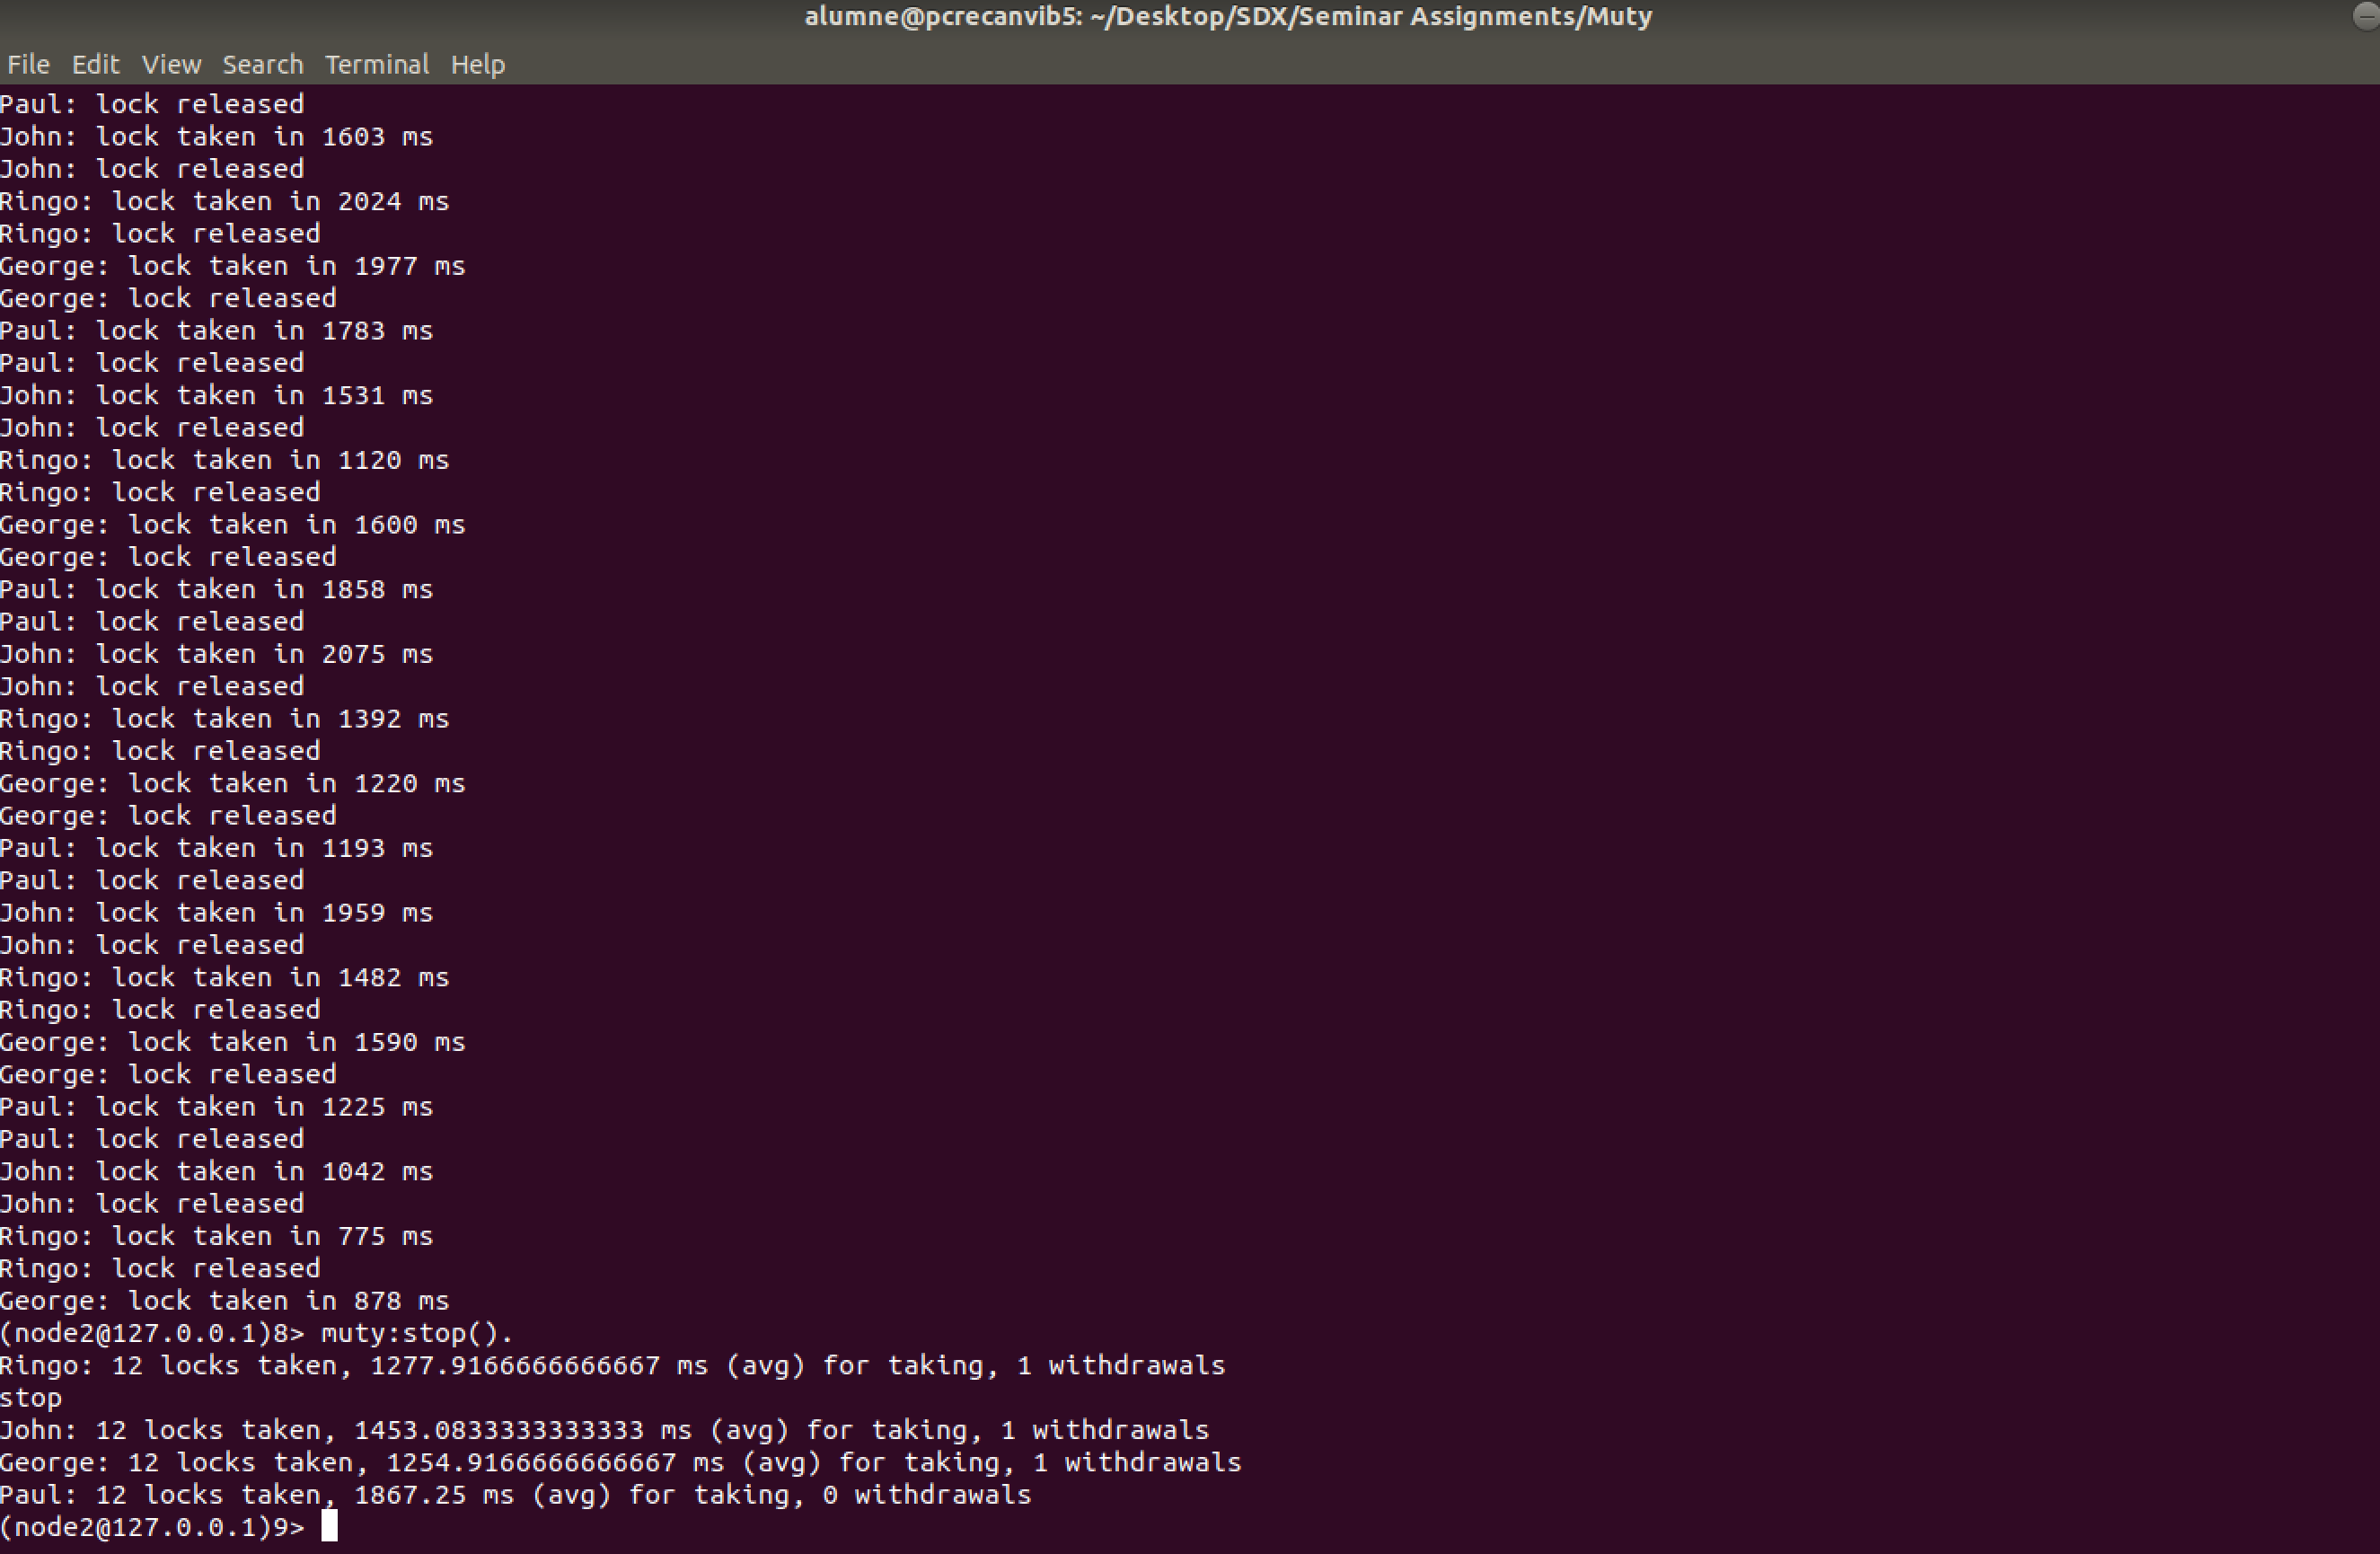
\includegraphics[width=\textwidth]{test-1}
\newpage També ens podem trobar amb la situació de que el temps de work, sigui més gran que el withdrawal time, per tant els workers a la espera superarien aquet temps. Tal i com podem observar:\\\\
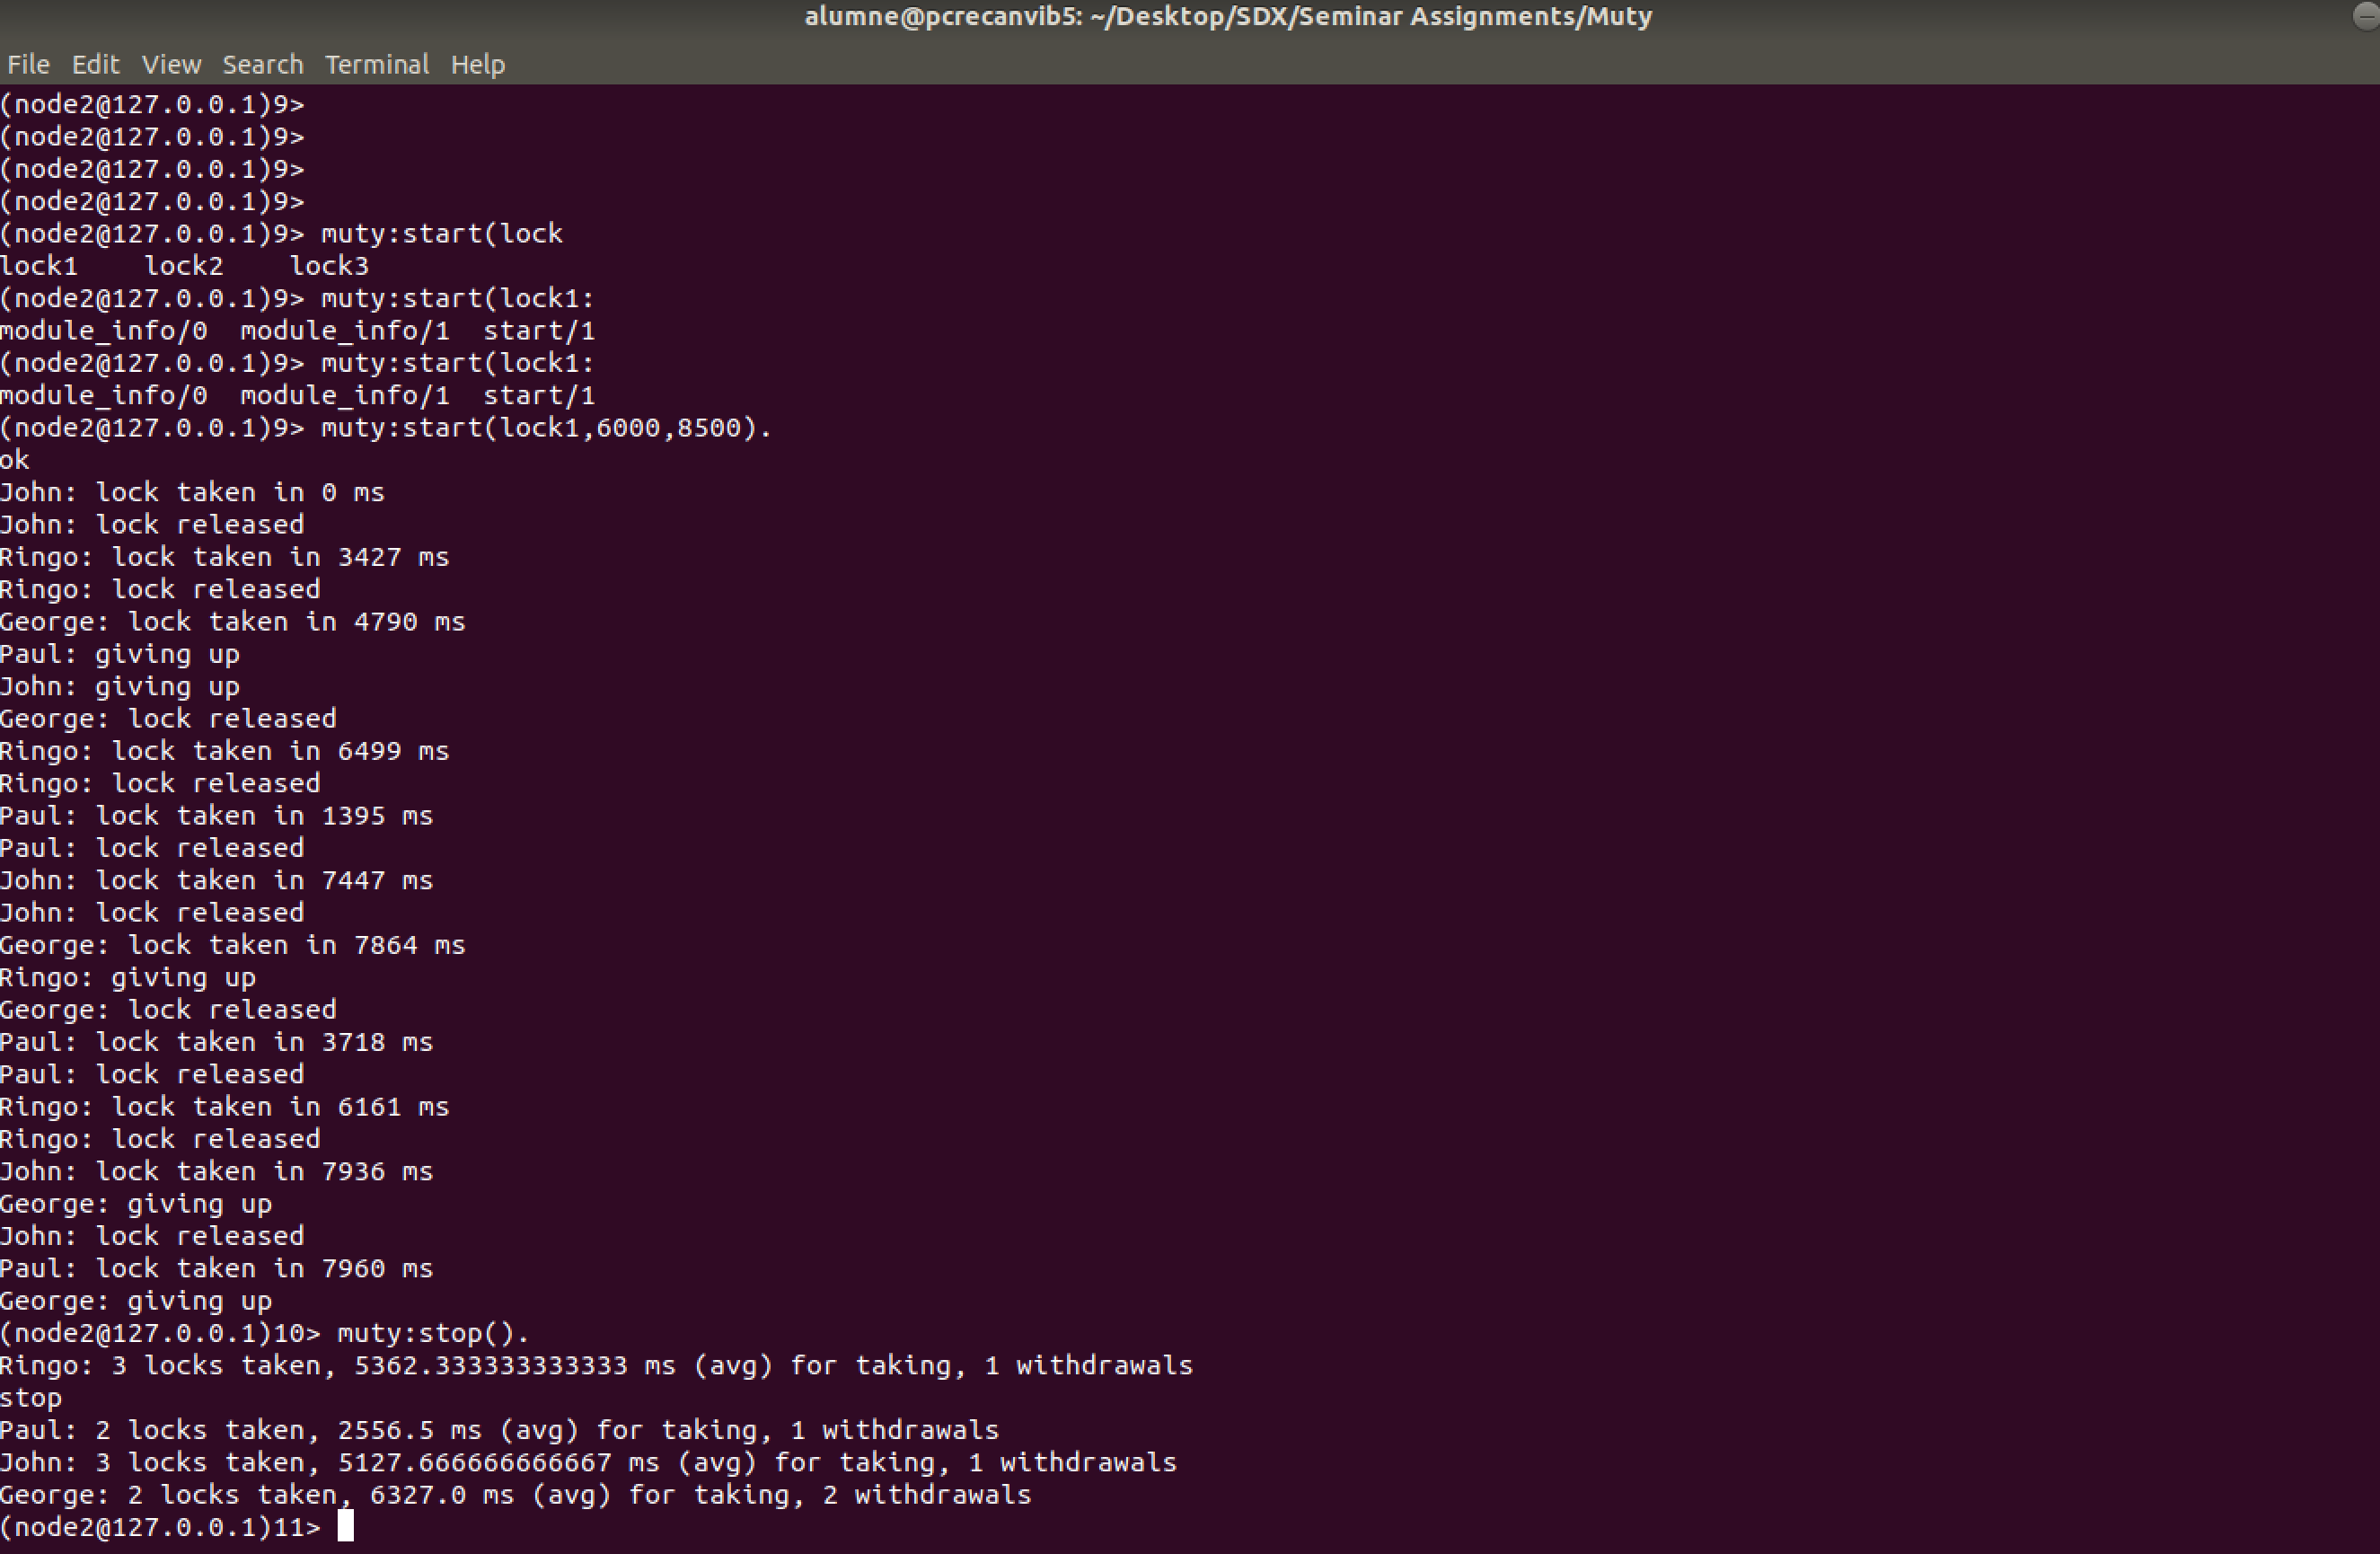
\includegraphics[width=\textwidth]{test-2}
\newpage\paragraph[bold]{Test 2: Sleep time superior a work time\\\\}
Si el temps de sleep, és més gran que el temps de work, estarem provocant, que les peticions d’accés a la regió critica dels diferents workers, estigui més espatllada, i per tant la possibilitat de trobar-nos en una situació de deadlock serà més baixa. Encara que no es una solució definitiva, ja que encara que essent menys probable també ens podem trobar amb una situació de deadlock, tal i com podem observar en la següent imatge:\\

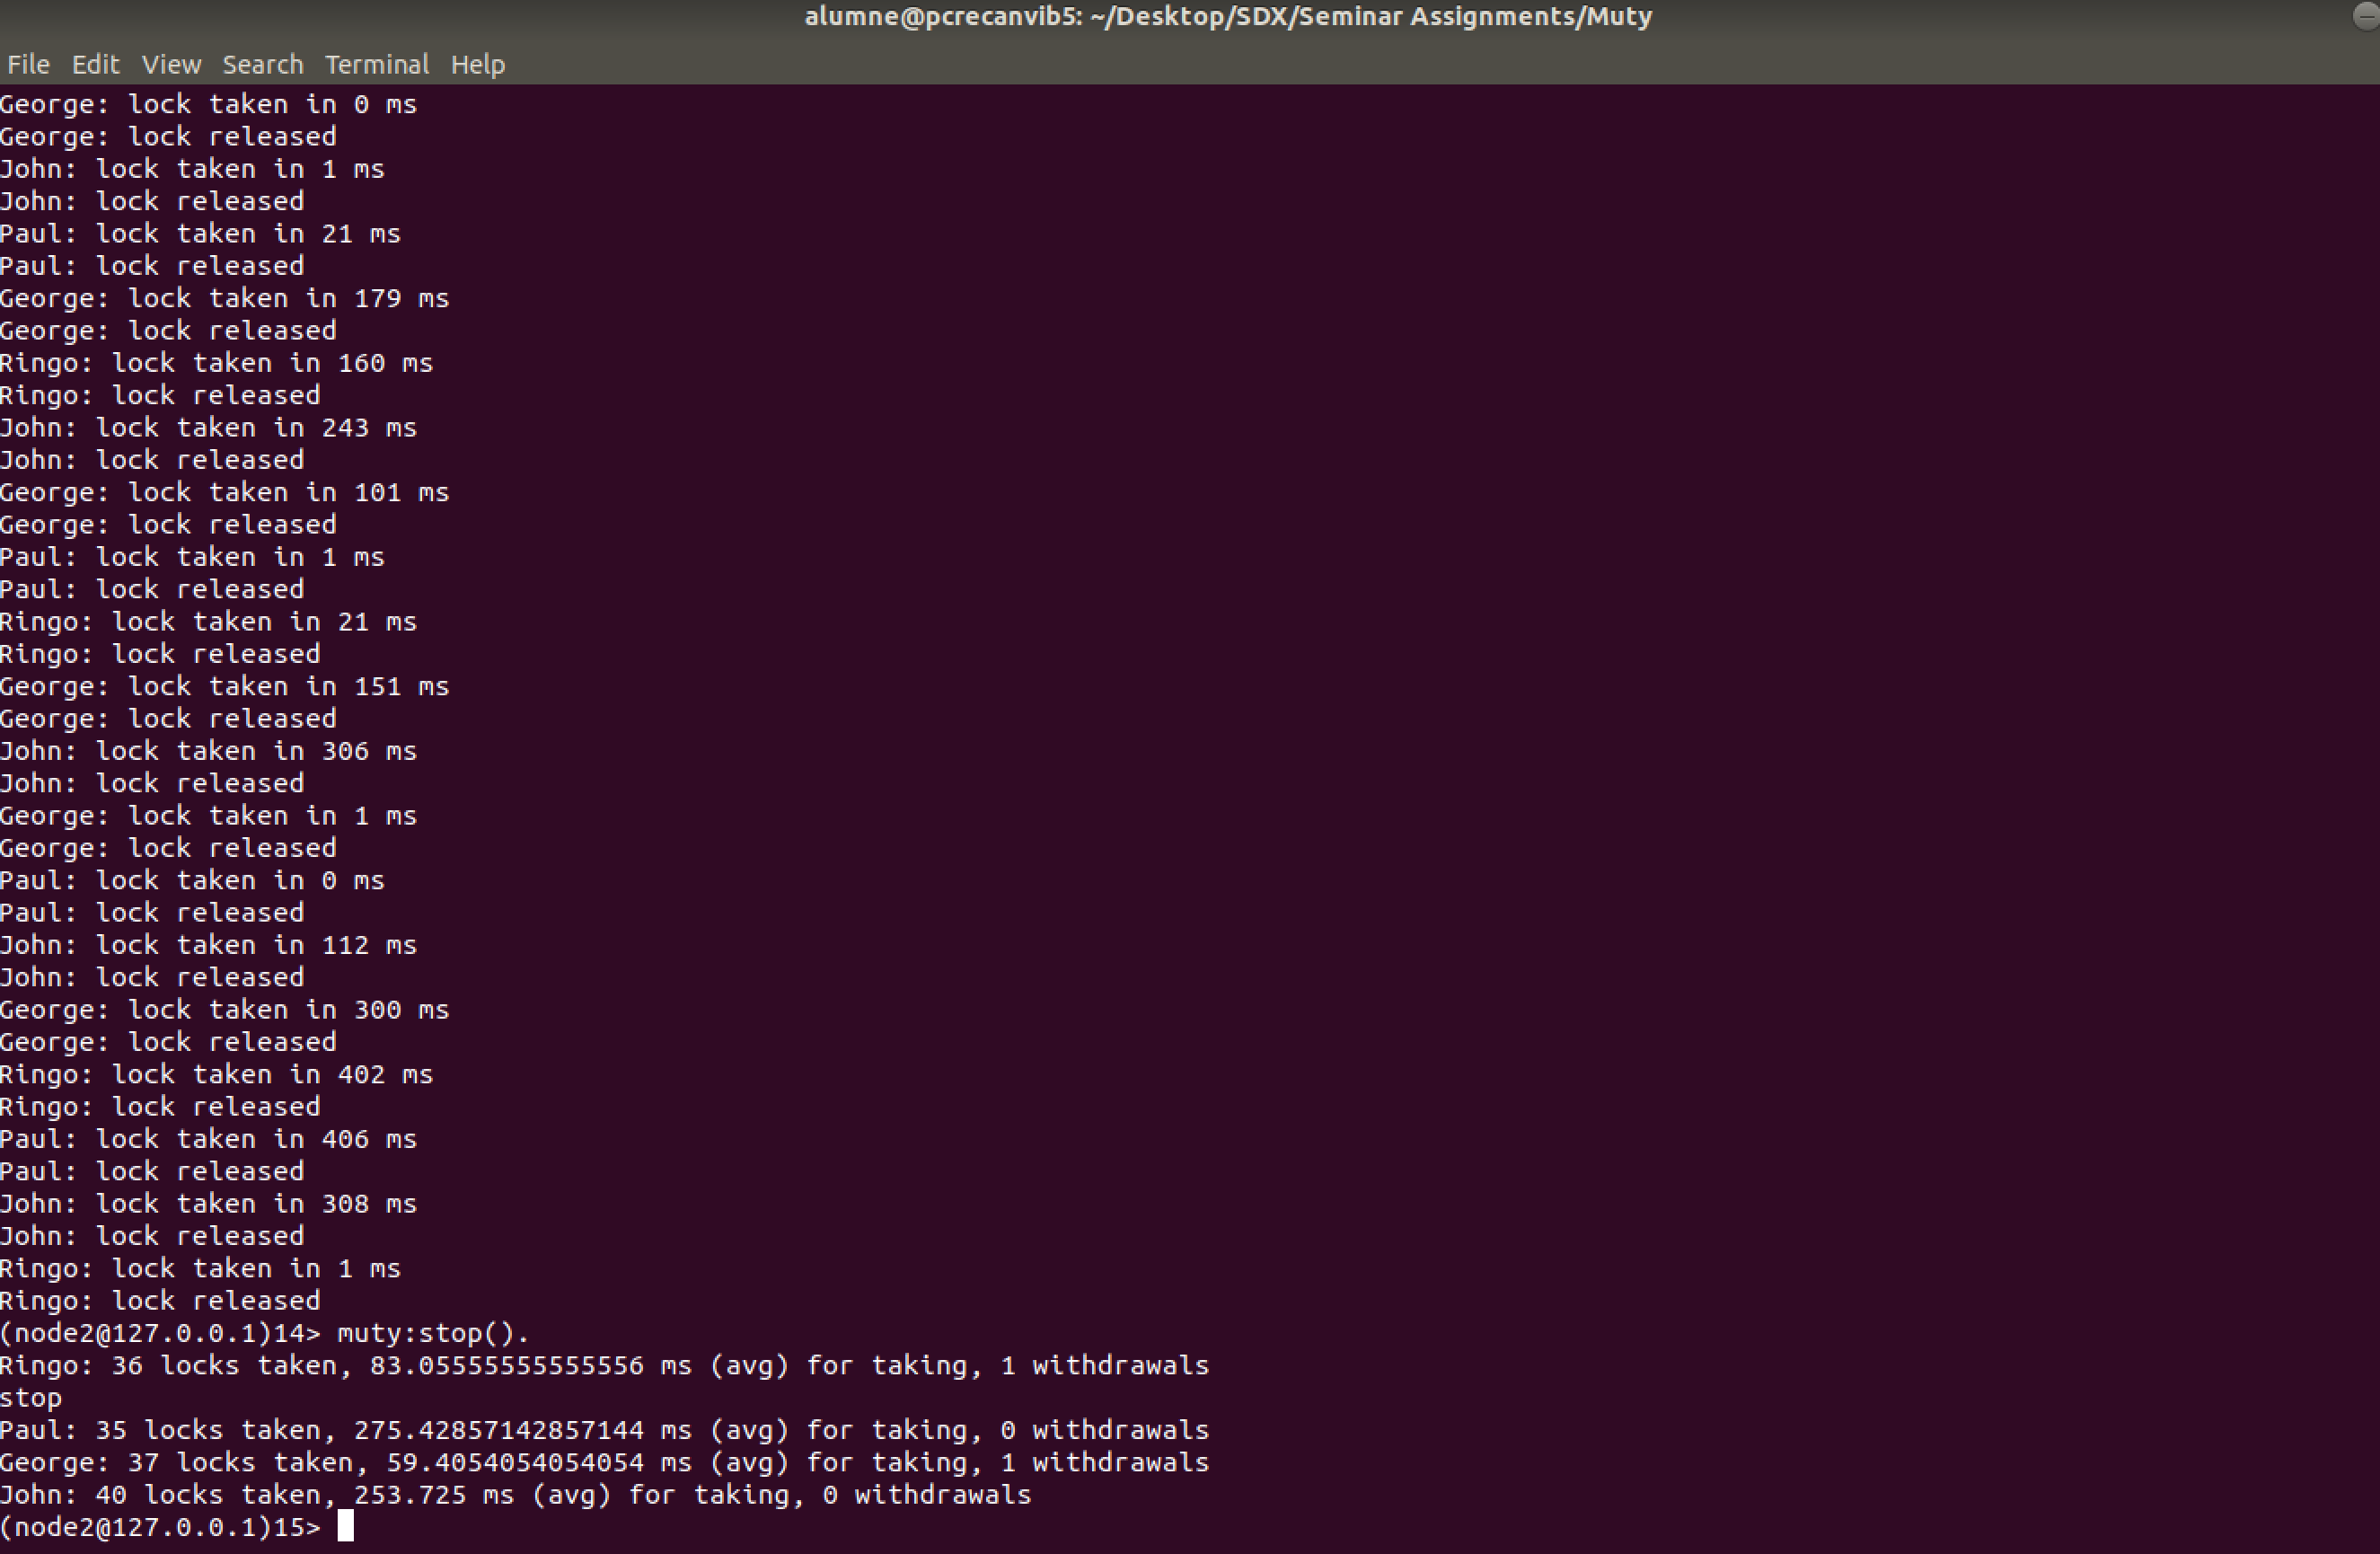
\includegraphics[width=\textwidth]{test-3}
\newpage
\paragraph[bold]{Test 3: Sleep time i work time iguals\\\\}

En aquesta situació, a la llarga també ens podriem trobar amb deadlocks, encara que  seran improbables com quan el sleep time es menor al work time. Ho podem observar en la següent imatge:\\

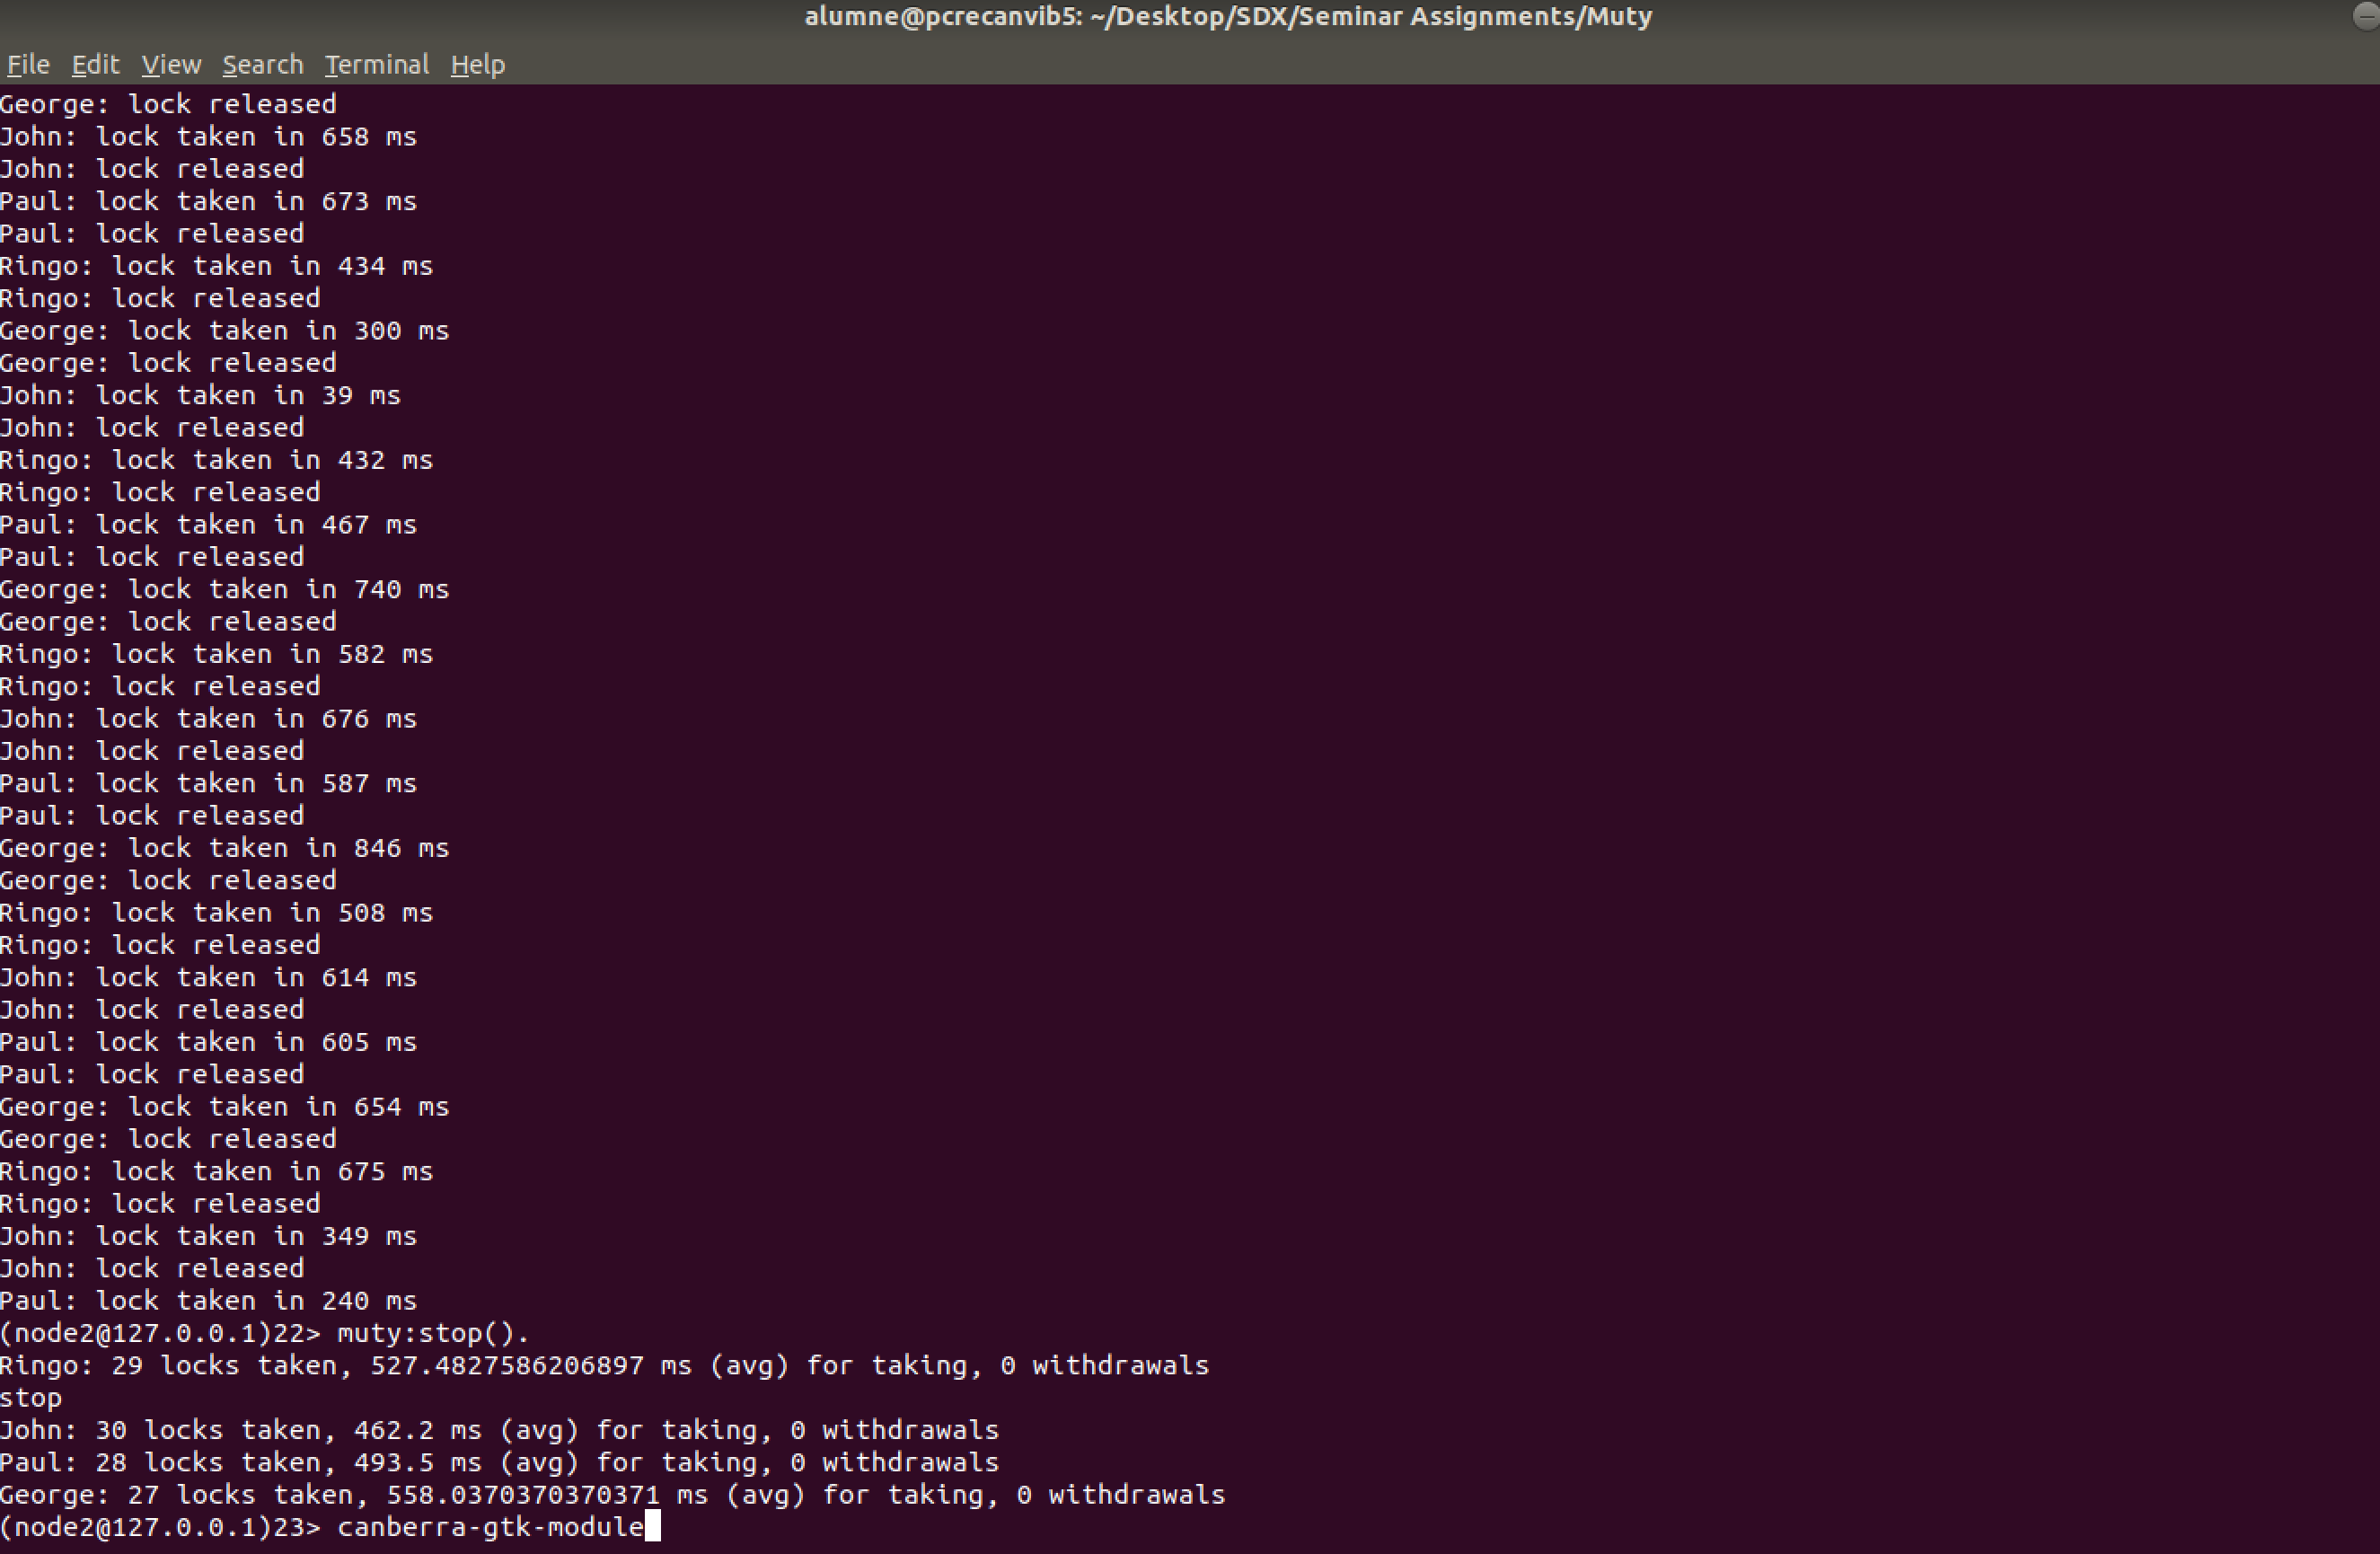
\includegraphics[width=\textwidth]{test-4}
\item Adapt the muty module to create each worker-lock pair in a different Erlang instance (that is, john and l1 should run in a node, ringo and l2 in another, and so on). Remember how processes are created remotely, how names registered in remote nodes are referred, and how Erlang runtime should be started to run distributed programs.\\\\
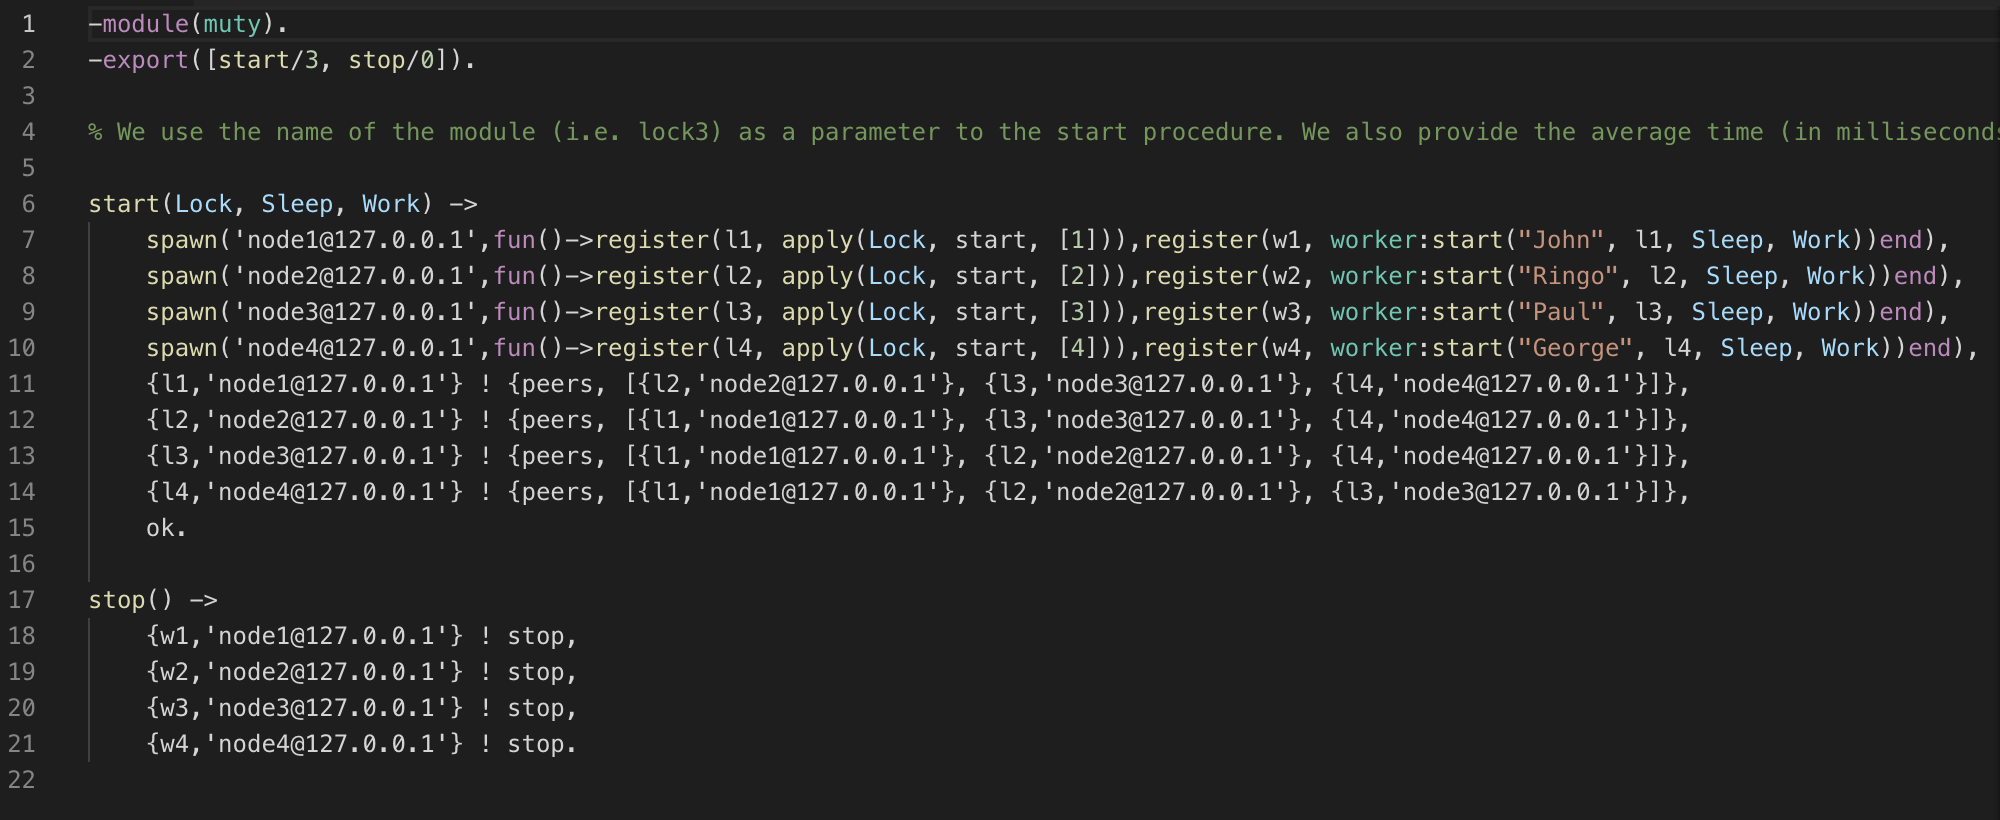
\includegraphics[width=\textwidth]{muty-code}

\end{enumerate}

\newpage\paragraph[bold]{Resolving deadlock}
\begin{enumerate}
\item Repeat the previous tests to compare the behavior of this lock with respect to the previous one.
\paragraph[bold]{Test 1: Sleep time inferior a work time}
\paragraph[bold]{Test 2: Sleep time superior a work time}
\paragraph[bold]{Test 3: Sleep time i work time iguals}
\end{enumerate}

\paragraph[bold]{Lamport’s time}
\begin{enumerate}
\item Repeat the previous tests to compare this version with the former ones.
\paragraph[bold]{Test 1: Sleep time inferior a work time}
\paragraph[bold]{Test 2: Sleep time superior a work time}
\paragraph[bold]{Test 3: Sleep time i work time iguals}
\end{enumerate}

\newpage
\section{Open questions}
\section{Personal opinion}
\end{document}